%! Licence = CC BY-NC-SA 4.0

%! Author = gianfluetsch
%! Date = 30. Dez 2021
%! Project = cydef_summary

\subsection{Volatility}
The \textit{Volatility Framework} is an open source, cross-platform, incident response framework that comes with many useful plugins that provide the investigator with a wealth of information from a snapshot of memory, also known as a memory dump. The concept of volatility has been around for a decade, and apart from analyzing running and hidden processes, it is also a very popular choice for malware analysis.

\subsubsection{Evidence}
\begin{itemize}
    \item Physical Memory
    \item Pagefile
    \item Crash Dumps
    \item Hibernation Files
\end{itemize}

\subsubsection{Volatility Artifacts}
\begin{itemize}
    \item Processes
    \item Network connections
    \item Loaded drivers
    \item Console command history
    \item Strings in memory
    \item Credentials and keys
    \item Everything running on a computer
\end{itemize}

\subsubsection{Process List}
\begin{itemize}
    \item Double linked list
    \item Process identification via iteration over each element
    \item Used by Windows Task Manager, tasklist, Get-Process cmdlet or pstree (Volatility)
\end{itemize}

\subsubsection{Hidden Process}
\begin{itemize}
    \item Detaching the process from the linked list hides it from standard tools
    \item psscan (Volatility)
\end{itemize}
\begin{center}
    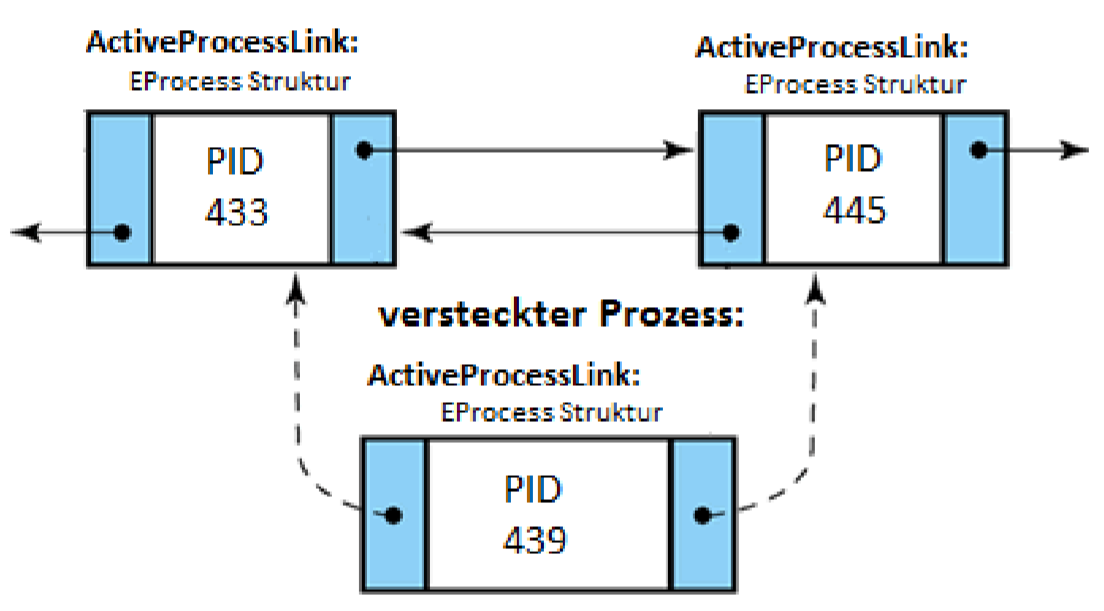
\includegraphics[width=1.0\linewidth]{./img/13-volatility/hidden_process}
    \vspace{-8pt}
\end{center}


\subsubsection{Creation of Memory Dumps}
To create a memory dump, several tools, such as \textit{Belkasoft Ram Capturer, FTK Imager, DD, DC3DD, Computer Aided INvestigative Environment (CAINE), Helix}, and \textit{Linux Memory Extractor (LiME)}, can be used to acquire the memory image or memory dump, and then be investigated and analyzed by the tools within the Volatility Framework.

\columnbreak

\subsubsection{imageinfo/ windows.info}
Let's figure out more information about the memory dump.

\textit{volatility2} is able to guess the OS (OS version of image), where \textit{volatiltiy3} was not finding the appropriate Windows kernel

\begin{lstlisting}[language=bash]
    volatility2 -f ./0zapftis.vmem imageinfo
    volatility3 -f ./0zapftis.vmem windows.info
\end{lstlisting}

\subsubsection{netscan (Network Scanner)}
This tool finds TCP endpoints, TCP listeners, UDP endpoints and UDP listeners.

\begin{lstlisting}[language=bash]
    volatility2 -f vmware-win-infected.vmem --profile Win10x64_10586 netscan
    volatility3 -f vmware-win-infected.vmem windows.netscan
\end{lstlisting}

\subsubsection{pslist - windows.pslist}
Let's figure out running processes

\begin{lstlisting}[language=bash]
    >volatility2 -f ./0zapftis.vmem pslist
    >volatility3 -f ./0zapftis.vmem windows.pslist

    Volatility 3 Framework 2.0.0
    Progress:  100.00		PDB scanning finished
    PID	PPID	ImageFileName	Offset(V)	Threads	Handles	SessionId	Wow64	CreateTime	ExitTime	File output

    4	0	System	0x819cc830	55	162	N/A	False	N/A	N/A	Disabled
    536	4	smss.exe	0x81945020	3	21	N/A	False	2011-10-10 17:03:56.000000 	N/A	Disabled
\end{lstlisting}

Looking at the above listing, nothing appears out of the ordinary. Although process alg.exe is present and can sometimes be used to indicate the presence of malware, as a lone indicator, it is not sufficient to warrant further investigation at this point as it is typically considered a legitimate Windows XP process. Perhaps the next plugin, psscan, will reveal more information.

\columnbreak

\subsubsection{pstree}
\textit{pstree} can be used to show the processes as a tree.

\begin{lstlisting}[language=bash]
    volatility2 -f vmware-win-infected.vmem --profile Win10x64_10586 pstree
    volatility3 -f vmware-win-infected.vmem windows.pstree
\end{lstlisting}

\subsubsection{psscan - windows.pscan}
Let's run psscan or windows.pscan

\begin{lstlisting}[language=bash]
    >volatility2 -f ./0zapftis.vmem psscan
    >volatility3 -f ./0zapftis.vmem windows.psscan

    Volatility 3 Framework 2.0.0
    Progress:  100.00		PDB scanning finished
    PID	PPID	ImageFileName	Offset	Threads	Handles	SessionId	Wow64	CreateTime	ExitTime	File output

    1616	676	alg.exe	0x156c5a0	7	99	0	False	2011-10-10 17:04:01.000000 	N/A	Disabled
    632	536	winlogon.exe	0x15a9020	24	533	0	False	2011-10-10 17:03:58.000000 	N/A	Disabled
\end{lstlisting}

Again, nothing appears particularly conspicuous. Moreover, this output looks very similar to the output of the pslist plugin. Perhaps the next plugin, psxview, will be of more assistance.

\subsubsection{psview - windows.psview}
Volatility provides an additional capability for detecting hidden running processes. The \textit{psxview} plugin provides a detailed listing of processes in a memory image by using five specific process detection methods. These include pslist, psscan, thrdproc, pspcdid and csrss. Moreover, the plugin makes use of physical memory addressing. For a process to be considered hidden, it should be invisible to, at a minimum, any non-csrss detection mechanism but may also be undetectable by subsequent process detection methods.

\begin{lstlisting}[language=bash]
    >volatility2 -f ./0zapftis.vmem psxview
    >Volatility 3: Does not include a direct psxview equivalent

    Volatility Foundation Volatility Framework 2.6.1
    Offset(P)  Name                    PID pslist psscan thrdproc pspcid csrss session deskthrd ExitTime
    ---------- -------------------- ------ ------ ------ -------- ------ ----- ------- -------- --------
    0x015a9020 winlogon.exe            632 True   True   True     True   True  True    True
\end{lstlisting}

Based on the plugin's output, no hidden processes were found for this memory image. Although some processes may be listed as hidden by the csrss method, they generally are not hidden. Therefore any process marked as hidden (FALSE) by this method requires that another method (pslist, psscan, thrdproc and pspcdid) confirm the suspicion. For Windows 7 and Vista systems, the list of internal processes is not available, and in some cases where Windows XP required memory pages might have been swapped out, the outcome of csrss may be affected.


\subsubsection{cmdscan}
The \textit{cmdscan} and consoles plugins may reveal additional information about commands typed into a command shell. The \textit{cmdscan} plugin is used to query the process memory of csrss.exe or conhost.exe for possible commands that may have been entered into the system shell (cmd.exe; i.e. PID 544) or through a backdoor or RDP session by an attacker. Specifically, it looks for COMMAND\_HISTORY based structures left behind in memory.

The \textit{consoles} plugin is similar to cmdscan, except that it searches for CONSOLE\_INFORMATION based data structures instead. More specifically, it provides the command history of commands fed to the system shell (cmd.exe; i.e. PID 544) or through backdoors and this data structure keeps both the input and output buffers for commands found using this plugin.

\begin{lstlisting}[language=bash]
    # cmdscan
    volatility2 -f ./0zapftis.vmem cmdscan
    # consoles
    volatility2 -f ./0zapftis.vmem consoles
    # cmdline
    volatility2 -f ./0zapftis.vmem cmdline
    volatility3 -f ./0zapftis.vmem windows.cmdline

    C:\Documents and Settings\Administrator>sc query malwar
    [SC] EnumQueryServicesStatus:OpenService FAILED 1060:
    The specified service does not exist as an installed service.

    C:\Documents and Settings\Administrator>sc query malware
    SERVICE_NAME: malware
            TYPE               : 1  KERNEL_DRIVER
            STATE              : 4  RUNNING
                                    (STOPPABLE,NOT_PAUSABLE,IGNORES_SHUTDOWN)
            WIN32_EXIT_CODE    : 0  (0x0)
            SERVICE_EXIT_CODE  : 0  (0x0)
            CHECKPOINT         : 0x0
            WAIT_HINT          : 0x0
\end{lstlisting}

Based on the output of these two plugins, some individual, either locally or remotely, queried the system for some service named malware. This service was found to be running and was found to be a kernel-based driver.

This information is a very important indicator of compromise as it provides several important clues. The first is that there appears to be a malicious driver on the system providing some unknown service, which is currently active. Moreover, any process initiated by this driver is not visible to Volatility’s process listing plugins (i.e. pslist, psscan and psxview). Thirdly, the service is known as malware. Taken together, these clues will help the investigator track down the malware.

\subsubsection{connscan}
The first network-based Volatility plugin that should be used is \textit{connscan}. It is used to verify the existence of ongoing network connections and scans a memory image for current or recently terminated connections. This plugin makes uses of physical memory addressing.

\begin{lstlisting}[language=bash]
    > volatility2 -f ./0zapftis.vmem connscan

    Volatility Foundation Volatility Framework 2.6.1
    Offset(P)  Local Address             Remote Address            Pid
    ---------- ------------------------- ------------------------- ---
    0x01a25a50 0.0.0.0:1026              172.16.98.1:6666          1956
\end{lstlisting}

Based on this information, PID 1956 (explorer.exe) has established a connection with remote system 172.16.98.1 using port 6666. This port is a well-known malware based port. The original IP address was 207.158.22.134 and was found communicating on port 443.

\columnbreak

\subsubsection{procdump}
\textit{procdump} can be used to dump the malicious process.

\begin{lstlisting}[language=bash]
    volatility2 -f vmware-win-infected.vmem --profile Win10x64_10586 procdump --pid 3496 --dump-dir .
    # volatility3 needs additional dependencies
    apt-get install capstone-tool python3-capstone
    volatility3 -f vmware-win-infected.vmem windows.dumpfiles --pid 3496
\end{lstlisting}

\subsection{Packed Malware}
\textit{Packed malware} has given malware creators and developers an opportunity for them to be able to bypass security systems such as antiviruses and anti-malware software that have been put in place by individuals and organizations to detect and capture malware and viruses.\\

To prevent detection and analysis of malware, malware developers use packers. A packer is a tool used to compress together data, resources and the executable files' code. It can also contain code for unpacking the program secretly and execute it.

Basically, packers help malware developers hide their malicious code. This code only gets unpacked and executed once the malware is executed. Apart from compressing malware, a packer can also be used to protect programs from cracking and copying.

\subsubsection{Encryption and packing tools}
There are a number of tools that can be used to pack and encrypt executable files. However, each of them serves a different purpose. Packers are not malicious on their own. Also, they were not created to hide malicious traits. Their main functionality is to compress executable files hence reducing their size. There are different types of packers. The most commonly used include:\\

\begin{itemize}
    \item \textbf{UPX (Ultimate Packer for Executables} — this is the most commonly used by malware developers. It is an open source and command-line tool. It also has the ability to unpack the packed files.
    \item \textbf{ASPack} — it has both a free and premium version. It was created to provide win32-exe file packing and protect it from reverse engineering.
\end{itemize}

\columnbreak

\subsubsection{Identifying a packed sample}

\textbf{Checking PE tool static signature}\\
This is the simplest and the easiest way. Here, you will try and identify if a malware is packed through the use of static signatures. It is important to note that every packer has unique characteristics that can assist you to easily identify it.\\

\textbf{Evaluating PE section headers}\\
The difference between a packed and unpacked PE file is that; an unpacked portable executable (PE) file contains the following sections \textit{.text, .code, .data, .idata, .rsrc} and \textit{.reloc} while a packed executable (for example one packed with upx) has section such as \textit{UPX0, UPX1, .aspack} among others.
With this, we can therefore conclude that after evaluating the section names of a PE file, you can identify one that is packed and one that is not. You can easily find the sections by opening the file in either PEiD or pestudio.\\

\textbf{Using stub execution signs}\\
As discussed earlier, most packers compress the PE file sections and then they add a new section at the end which contains the unpacking code (stub). Most unpacked PE files start their execution from the first section which is either \textit{.text} or \textit{.code}. However, the packed files will always start their execution from one of the last sections. This is a clear indication that there is a decryption process underway.